\begin{task}
\TT{Oblicz moc i wartość skuteczną sygnału okresowego $f(t)$ przedstawionego na rysunku: }{Calculate the average power and the effective value (RMS) for the periodic signal $f(t)$ given below:}

\begin{figure}[H]
\centering
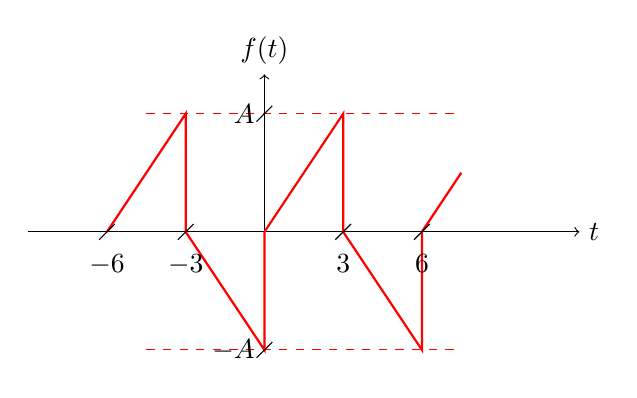
\begin{tikzpicture}
  %\draw (0,0) circle (1in);
  \draw[->] (-3.0,+0.0) -- (4.0,+0.0) node[right] {$t$};
  \draw[->] (+0.0,-1.5) -- (+0.0,+2.0) node[above] {$f(t)$};
  \draw[-,red, thick] (-2.0,0.0) -- (-1.0,1.5)--(-1.0,0.0) -- (0.0,-1.5) -- (0.0,+0.0) -- (+1.0,+1.5) -- (+1.0,+0.0) -- (+2.0,-1.5) -- (+2.0,+0.0) -- (2.5,0.75);
  \draw[-,red, dashed] (-1.5,1.5) -- (2.5,1.5);
  \draw[-,red, dashed] (-1.5,-1.5) -- (2.5,-1.5);

  \draw[-] (-2.0-0.1,-0.1)--(-2.0+0.1,0.1) node[midway, below, outer sep=5pt] {$-6$};
  \draw[-] (-1.0-0.1,-0.1)--(-1.0+0.1,0.1) node[midway, below, outer sep=5pt] {$-3$};
  \draw[-] (+1.0-0.1,-0.1)--(+1.0+0.1,0.1) node[midway, below, outer sep=5pt] {$3$};
  \draw[-] (+2.0-0.1,-0.1)--(+2.0+0.1,0.1) node[midway, below, outer sep=5pt] {$6$};
  \draw[-] (-0.1,+1.5-0.1)--(+0.1,+1.5+0.1) node[midway, left] {$A$};
  \draw[-] (-0.1,-1.5-0.1)--(+0.1,-1.5+0.1) node[midway, left] {$-A$};

\end{tikzpicture}
\end{figure}

\TT{W pierwszej kolejności należy ustalić wzór funkcji przedstawionej na rysunku. Jest to funkcja przedziałowa. W pierwszym okresie możemy ją opisać za pomocą dwóch prostych. Ogólne równanie prostej to:}{First of all, the definition of $f(t)$ signal has to be derived. This is periodic piecewise function, piecewise linear function to be precise.
The simplest form of linear function is:}

\begin{equation}
f(t) = a \cdot t + b
\end{equation}

\TT{W pierwszym okresie, w pierwszej części, wykres funkcji jest prostą przechodzącą przez dwa punkty: $(0,0)$ oraz $(3,A)$. Możemy więc napisać układ równań, rozwiązać go i znaleźć nieznane parametry $a$ i $b$. }{In the first interval of the first period (i.e. $t \in (0; 3)$), linear function crosses two points: $(0,0)$ and $(3,A)$. So, in order to derive $a$ and $b$, the following system of the equations has to be solved.}  

\begin{align*}
&\left\{\begin{matrix*}[l]
0 = a\cdot 0 +b\\ 
A = a\cdot 3 +b
\end{matrix*}\right. \\
&\left\{\begin{matrix*}[l]
0 = b\\ 
A = a \cdot 3 +b
\end{matrix*}\right. \\
&\left\{\begin{matrix*}[l]
0 = b\\ 
A = a \cdot 3 +0
\end{matrix*}\right. \\
&\left\{\begin{matrix*}[l]
0 = b\\ 
\frac{A}{3} = a
\end{matrix*}\right.
\end{align*}

\TT{Podsumowując, pierwszy odcinek funkcji przedstawionej na rysunku, w pierwszym okresie można opisać wzorem:}{As a result we get:}
\begin{align*}
f(t) = \frac{A}{3}\cdot t
\end{align*}

\TT{Drugi odcinek funkcji jest prostą przechodzącą przez następujące dwa punkty: $(3,0)$ oraz $(6,-A)$. Możemy więc napisać układ równań, rozwiązać go i znaleźć nieznane parametry $a$ i $b$.}{In the second interval of the first period (i.e. $t \in (3; 6)$), linear function crosses other two points:: $(3,0)$ and $(6,-A)$. So, in order to derive $a$ and $b$, the following system of the equations has to be solved.}

\begin{align*}
&\left\{\begin{matrix*}[l]
0 = a\cdot 3 +b\\ 
-A = a\cdot 6 +b
\end{matrix*}\right. \\
&\left\{\begin{matrix*}[l]
-3 \cdot a = b\\ 
-A = 6 \cdot a -3 \cdot a
\end{matrix*}\right. \\
&\left\{\begin{matrix*}[l]
-3 \cdot a = b\\ 
-A = 3 \cdot a
\end{matrix*}\right. \\
&\left\{\begin{matrix*}[l]
-3 \cdot a = b\\  
-\frac{A}{3} = a
\end{matrix*}\right. \\
&\left\{\begin{matrix*}[l]
-3 \cdot (-\frac{A}{3}) = b\\
-\frac{A}{3} = a
\end{matrix*}\right. \\
&\left\{\begin{matrix*}[l]
A = b\\
-\frac{A}{3} = a
\end{matrix*}\right.
\end{align*}

\TT{A więc drugi odcinek funkcji przedstawionej na rysunku w pierwszym okresie, można opisać wzorem:}{As a result, second interval of the first period is described by:}

\begin{align*}
f(t) = -\frac{A}{3}\cdot t + A
\end{align*}

\TT{W związku z tym, całą funkcję w pierwszym okresie można zapisać jako funkcje przedziałową:}{As a result the piecewise linear function in the first period is given by:}

\begin{align*}
f(t) = \left\{\begin{matrix*}[l]
\frac{A}{3}\cdot t & for &t \in (0;3)\\ 
-\frac{A}{3}\cdot t + A & for & t \in (3; 6)
\end{matrix*}\right.
\end{align*}

\TT{I ogólniej, całą funkcję można wyrazić następującym wzorem:}{For the whole periodic signal $f(t)$ we get:}

\begin{align*}
f(t) = \left\{\begin{matrix*}[l]
\frac{A}{3}\cdot \left( t - k\cdot 6 \right) & for &t \in (0 + k\cdot 6; 3 + k\cdot 6)\\ 
-\frac{A}{3}\cdot \left( t - k\cdot 6 \right) + A & for & t \in (3 + k \cdot 6; 6+ k\cdot 6)
\end{matrix*}\right. \wedge k \in \TT{I}{Z}
\end{align*}

\TT{Moc sygnału okresowego wyznaczamy ze wzoru:}{The average power for periodic signals is defined by:}

\begin{equation}
P=\frac{1}{T} \cdot \int_{T}^{}\left|f(t)\right|^2 \cdot dt
\end{equation}

\TT{Podstawiamy do wzoru na moc wzór naszej funkcji:}{In our case we get:}

\begin{align*}
P&=\frac{1}{T} \cdot \int_{T}^{}\left|f(t)\right|^2 \cdot dt=\\
 &=\frac{1}{6} \cdot \left( \int_{0}^{3}\left|\frac{A}{3}\cdot t \right|^2 \cdot dt
  +\int_{3}^{6}\left|-\frac{A}{3}\cdot t + A\right|^2 \cdot dt \right)=\\ 
 &=\frac{1}{6} \cdot \int_{0}^{3}\left(\frac{A}{3}\cdot t \right)^2 \cdot dt
  +\frac{1}{6} \cdot \int_{3}^{6}\left(-\frac{A}{3}\cdot t + A\right)^2 \cdot dt=\\ 
 &=\frac{1}{6} \cdot \int_{0}^{3}\frac{A^2}{9}\cdot t^2 \cdot dt
 +\frac{1}{6} \cdot \int_{3}^{6}\left(\left(-\frac{A}{3}\cdot t\right)^2 - 2\cdot \frac{A}{3}\cdot t \cdot  A + A^2 \right) \cdot dt=\\ 
 &=\frac{A^2}{54}\cdot \int_{0}^{3} t^2 \cdot dt
 +\frac{1}{6} \cdot \int_{3}^{6}\frac{A^2}{9}\cdot t^2 \cdot dt - \frac{1}{6} \cdot \int_{3}^{6} \frac{2 \cdot A^2}{3}\cdot t \cdot dt + \frac{1}{6} \cdot \int_{3}^{6} A^2 \cdot dt=\\
 &=\frac{A^2}{54}\cdot \left. \frac{t^3}{3} \right|_{0}^{3}
 +\frac{A^2}{54}\cdot \int_{3}^{6} t^2 \cdot dt - \frac{2 \cdot A^2}{18}\cdot \int_{3}^{6} t^2 \cdot dt +\frac{A^2}{6}\cdot \int_{3}^{6} dt=\\
 &=\frac{A^2}{162}\cdot \left(3^3 - 0^3\right) + \frac{A^2}{54}\cdot \left. \frac{t^3}{3} \right|_{3}^{6} - \frac{2 \cdot A^2}{18}\cdot \left. \frac{t^2}{2} \right|_{3}^{6} + \frac{A^2}{6}\cdot \left. t \right|_{3}^{6}=\\
 &=\frac{A^2}{162}\cdot 27 + \frac{A^2}{162}\cdot \left(6^3 - 3^3\right) - \frac{2 \cdot A^2}{36}\cdot \left(6^2 - 3^2\right) + \frac{A^2}{6}\cdot (6-3)=\\
 &=\frac{A^2}{6} + \frac{A^2}{162}\cdot 189 - \frac{2 \cdot A^2}{36}\cdot 27 + \frac{A^2}{6}\cdot 3=\\
 &=\frac{A^2}{6} + \frac{7 \cdot A^2}{6} - \frac{9 \cdot A^2}{6} + \frac{3 \cdot A^2}{6}=\\
 &=\frac{2 \cdot A^2}{6}=\\
 &=\frac{A^2}{3}
\end{align*}

\TT{Moc sygnału równa się $\frac{A^2}{3}$.}{The average power equals to $\frac{A^2}{3}$.}

\TT{Wzór na obliczenie wartości skutecznej to:}{The effective value (RMS) is defined by:}
\begin{equation}
RMS=\sqrt P
\end{equation}

\TT{Wartość skuteczna sygnału to $\frac{A}{\sqrt 3}$.}{Therefore, effective value (RMS) equals to $\frac{A}{\sqrt 3}$.}
\end{task}